\documentclass[10pt,journal,compsoc]{IEEEtran}

\usepackage[utf8]{inputenc}
\usepackage[spanish,es-nodecimaldot,english]{babel}
\usepackage{amsmath,amssymb,amsfonts}
\usepackage{booktabs}
\usepackage{graphicx}
\usepackage{cite}
\usepackage{url}
\usepackage{hyperref}
\usepackage{xcolor}
\usepackage{microtype}
\usepackage{tabularx}
\usepackage{subcaption}

\hypersetup{
    colorlinks=true,
    linkcolor=blue,
    citecolor=blue,
    urlcolor=blue,
    pdftitle={Evaluacion Experimental y Adaptacion Supervisada de Laya Multilingual: Triaje de Incidentes de Service Desk mediante Modelos de Decision System-1},
    pdfauthor={Juan Retamales}
}

\begin{document}

\title{Evaluaci\'on Experimental y Adaptaci\'on Supervisada de Laya Multilingual: Triaje de Incidentes de Service Desk mediante Modelos de Decisi\'on System-1}

\author{Juan~Retamales%
\thanks{J. Retamales es Ingeniero e Investigador Principal en Tecnolog\'{\i}as de la Informaci\'on e Inteligencia Artificial aplicada a la gesti\'on de operaciones de Service Desk. Contacto: \texttt{juan.retamales@example.org}. Repositorio del proyecto: \url{https://github.com/juanretamales/laya-service-desk}}%
}

\markboth{IEEE Transactions on Systems, Man, and Cybernetics / ArXiv Preprint, Noviembre~2026}%
{Retamales: Evaluaci\'on Experimental y Adaptaci\'on de Laya para Triaje de Service Desk}

\IEEEtitleabstractindextext{%
\begin{otherlanguage}{english}
\begin{abstract}
Automating IT Service Desk incident triage requires fast, reliable, and deterministic categorization to minimize reassignment delays without incurring prohibitive computational costs. While Large Language Models (LLMs) offer high linguistic flexibility, their autoregressive nature imposes significant latency (1--5 seconds per ticket), high operational expense, and the constant hazard of textual hallucination. In this work, we investigate the application and supervised fine-tuning of \textbf{Laya Multilingual} (a 322M-parameter, open-weight Foundation Model based on mmBERT/XLM-RoBERTa) operating as a discriminative \emph{System-1 Decision Model}. Rather than generating unstructured text, Laya resolves multiple structured operational queries (\texttt{category}, \texttt{priority}, \texttt{support\_group}) in a single forward pass. Evaluated on an immutable, leak-free test partition of enterprise IT support tickets in Spanish (217 tickets, SHA-256 verified), the unadapted base checkpoint in Zero-Shot mode achieved an unsatisfactory category accuracy of only \textbf{18.89\%} (Macro-F1: 18.57\%), severely handicapped by lexical priors over domain definitions. Following supervised multi-task fine-tuning with early stopping, our adapted model attained \textbf{83.56\% category accuracy} (Macro-F1: 83.40\%), representing a net gain of \textbf{+64.67 percentage points} and a \textbf{4.42$\times$ relative performance multiplier}. With a compact memory footprint of $\sim$1.28~GB, millisecond CPU/GPU latency, and zero generative hallucination, our findings demonstrate that localized System-1 decision models represent an optimal, cost-effective paradigm for mission-critical enterprise helpdesk automation.
\end{abstract}
\begin{IEEEkeywords}
IT Service Desk, System-1 Decision Models, Laya Multilingual, Incident Triage, Supervised Fine-Tuning, Calibration, Selective Escalation.
\end{IEEEkeywords}
\end{otherlanguage}

\vspace{0.5em}
\begin{abstract}
El triaje automatizado de incidentes en mesas de ayuda (IT Service Desk) exige una categorizaci\'on r\'apida, determinista y confiable que minimice los retrasos de reasignaci\'on sin incurrir en costes computacionales desproporcionados. Aunque los modelos de lenguaje autorregresivos masivos ofrecen gran versatilidad, introducen latencias elevadas (1--5 segundos por ticket), elevados costes por inferencia y el riesgo persistente de alucinaci\'on. En este art\'{\i}culo, evaluamos la adaptaci\'on supervisada de \textbf{Laya Multilingual} (322M par\'ametros, licencia Apache-2.0) operando bajo el paradigma de \emph{Modelos de Decisi\'on System-1}. Laya proyecta el estado contextual del ticket hacia m\'ultiples consultas tipadas estructuradas en una sola pasada hacia adelante (\emph{single forward pass}). Evaluado sobre una partici\'on de prueba inmutable de tickets en espa\~nol (217 tickets congelados con hash SHA-256 y 0\% de fuga), el modelo base original en modo Zero-Shot registr\'o una exactitud de apenas \textbf{18.89\%} (Macro-F1: 18.57\%), lastrado por la dominancia de sesgos l\'exicos. Tras el ajuste supervisado con parada temprana, el modelo alcanz\'o una \textbf{exactitud global de 83.56\%} (Macro-F1: 83.40\%), lo que representa una ganancia neta de \textbf{+64.67 puntos porcentuales} (mejora de \textbf{4.42$\times$}). Con un tama\~no en disco de $\sim$1.28~GB, latencia de milisegundos y nula alucinaci\'on, demostramos la superioridad y viabilidad de los modelos de decisi\'on tipados para operaciones empresariales cr\'{\i}ticas.
\end{abstract}
\begin{IEEEkeywords}
Service Desk, Modelos de Decisi\'on System-1, Laya Multilingual, Triaje de Incidentes, Fine-Tuning Supervisado, Calibraci\'on, Escalamiento Selectivo.
\end{IEEEkeywords}
}

\maketitle
\IEEEdisplaynontitleabstractindextext
\IEEEpeerreviewmaketitle

\section{Introducci\'on}
\IEEEPARstart{E}{n} la gesti\'on de servicios de tecnolog\'{\i}as de la informaci\'on (ITSM) conforme a las directrices de ITIL 4 \cite{itil4_foundation}, el \emph{Service Desk} representa el punto \'unico de contacto operativo entre los usuarios finales y la infraestructura corporativa. Una de las actividades m\'as cr\'{\i}ticas en este flujo es el \textbf{triaje y enrutamiento inicial de incidentes}: clasificar el incidente en la categor\'{\i}a t\'ecnica correcta (e.g., Software, Hardware, Acceso, Correo Electr\'onico), asignarle una prioridad operativa y derivarlo al grupo resolutor competente.

Cualquier error de asignaci\'on introduce el fen\'omeno conocido como \emph{ticket bouncing} (rebote continuo entre \'areas resolutoras), lo que degrada sustancialmente los acuerdos de nivel de servicio (SLA) y encarece la operaci\'on. Hist\'oricamente, la automatizaci\'on del triaje dependi\'o de reglas manuales basadas en palabras clave o clasificadores de aprendizaje superficial (SVM, Naive Bayes), incapaces de capturar la ambig\"uedad sem\'antica natural del usuario corporativo.

Recientemente, el despliegue de grandes modelos de lenguaje (LLMs) generativos ha pretendido resolver esta carencia. No obstante, como identifican Li \cite{li2026fast} y Nandakishore \cite{nandakishore2026laya}, los LLMs generativos sufren de tres limitaciones fundamentales en entornos de soporte cr\'{\i}tico:
\begin{enumerate}
    \item \textbf{Latencia autorregresiva:} La generaci\'on token a token demanda entre 1 y 5 segundos por petici\'on, creando cuellos de botella en colas de tickets de alta concurrencia.
    \item \textbf{Riesgo de alucinaci\'on:} Al generar texto libre, los modelos generativos pueden sugerir categor\'{\i}as inexistentes o inventar instrucciones resolutorias sin base f\'actica.
    \item \textbf{Sobrecosto computacional:} Requieren hardware masivo (m\'ultiples GPUs de 24--80~GB de VRAM) para tareas que en esencia son decisiones discriminativas acotadas.
\end{enumerate}

Para superar esta disyuntiva, surge el paradigma de los \textbf{Modelos de Decisi\'on System-1} (\emph{System-1 Decision Models}) \cite{li2026fast, nandakishore2026laya}. Inspirados en la teor\'{\i}a dual del procesamiento cognitivo, los modelos System-1 resuelven preguntas estructuradas y tipadas en una sola pasada de inferencia (\emph{single forward pass}), devolviendo una distribuci\'on de probabilidad sobre un conjunto cerrado de opciones operacionales.

Entre estas arquitecturas destaca \textbf{Laya Multilingual} \cite{convai2026laya}, un codificador fundacional abierto de 322 millones de par\'ametros derivado de XLM-RoBERTa / mmBERT \cite{conneau2020unsupervised, clark2024modernbert}. Laya implementa de forma nativa cabezales de decisi\'on tipada (\texttt{choice}, \texttt{score}, \texttt{noul}) optimizados mediante Aprendizaje por Refuerzo a partir de Decisiones Conversacionales (RLCD).

En este art\'{\i}culo, presentamos la primera investigaci\'on emp\'{\i}rica exhaustiva de la aplicaci\'on y adaptaci\'on supervisada de Laya Multilingual para la gesti\'on de tickets de soporte en idioma espa\~nol. Nuestros principales aportes son:
\begin{itemize}
    \item \textbf{Evaluaci\'on emp\'{\i}rica Zero-Shot:} Medimos el desempe\~no del checkpoint base \texttt{convaiinnovations/laya-multilingual} sobre un banco de prueba congelado de 217 tickets corporativos en espa\~nol, evidenciando un rendimiento de exactitud de solo 18.89\%, y formalizando las causas te\'oricas de este fen\'omeno a partir de la dominancia de etiquetas sobre definiciones analizada por Azizi et al. \cite{azizi2026labels}.
    \item \textbf{Protocolo de adaptaci\'on supervisada y convergencia:} Implementamos un ajuste supervisado multitarea con aislamiento estricto de particiones (0\% fuga, validaci\'on inmutable), logrando una exactitud de \textbf{83.56\%} (+64.67 pp, factor 4.42$\times$).
    \item \textbf{An\'alisis de calibraci\'on y escalamiento selectivo:} Fundamentamos una pol\'{\i}tica de escalamiento y compuertas de seguridad basada en los trabajos de Nandakishore \cite{nandakishore2026laya}, Lu y Wu \cite{lu2026benchmarking} y Brom \cite{brom2026confidence}, garantizando una integraci\'on segura en entornos empresariales.
\end{itemize}

---

\section{Trabajos Relacionados y Marco Te\'orico}

\subsection{Modelos de Decisi\'on Tipados y la Dicotom\'{\i}a System-1 / System-2}
El an\'alisis de arquitecturas de decisi\'on en agentes y sistemas de producci\'on ha sido formalizado recientemente por Li \cite{li2026fast}, quien define a los modelos de decisi\'on System-1 como clasificadores discriminativos contextuales que reciben el estado operacional $S$ y un esquema tipado de preguntas $Q=\{q_1, \dots, q_k\}$, devolviendo un vector de probabilidad $p \in \Delta^{|C|}$ sobre un conjunto cerrado de opciones $C$. A diferencia de los modelos generativos System-2 (e.g., Llama-3, Qwen-2.5-7B), los modelos System-1 no emiten texto token a token, sino que eval\'uan simult\'aneamente la afinidad entre la representaci\'on contextual del texto y las representaciones latentes de los criterios de decisi\'on.

Esta arquitectura fue popularizada inicialmente por Jev \cite{li2026fast, azizi2026labels} como un servicio cerrado de enrutamiento y triaje. Laya \cite{convai2026laya} constituye su contraparte formal de pesos abiertos, implementada sobre codificadores modernos tipo Transformer \cite{clark2024modernbert} con cabezales dedicados a preguntas categ\'oricas (\texttt{choice}) y cuantitativas (\texttt{score}).

\subsection{El Fen\'omeno ``Labels Override Definitions''}
Un interrogante crucial al emplear modelos de decisi\'on en modo Zero-Shot es el grado en que el modelo respeta las reglas y descripciones textuales frente a los nombres literales de las etiquetas. Azizi et al. \cite{azizi2026labels} demostraron experimentalmente que los modelos tipados de la familia Jev/Laya exhiben una fuerte tendencia a ignorar las definiciones detalladas si entran en conflicto con la sem\'antica previa del nombre de la etiqueta (\emph{label bias}). 

En el contexto de Service Desk, t\'erminos t\'ecnicos como ``Acceso'' o ``Software'' poseen definiciones precisas de acuerdo a ITIL (e.g., restablecimiento de credenciales VPN vs. fallo de instalaci\'on de un ejecutable). Como demostraremos en la Secci\'on~V, el checkpoint base sin ajustar colapsa ante estas diferencias sutiles, ratificando la necesidad ineludible del ajuste supervisado de dominio.

\subsection{Adaptaciones de Dominio Cr\'{\i}ticas de Laya}
El potencial de Laya para tareas cr\'{\i}ticas ha sido corroborado en dominios especializados de alta exigencia:
\begin{itemize}
    \item \textbf{Operaciones Satelitales (SatOps):} Mei et al. \cite{mei2026satops} desarrollaron \emph{SatOps-Decision}, adaptando localmente un codificador Laya para decisiones de comunicaciones a bordo de sat\'elites. Demostraron que el modelo ajustado alcanz\'o un 85.3\% de exactitud con latencias de 90~ms frente a los 493~ms de modelos generativos livianos (speedup de 5.47$\times$).
    \item \textbf{Triaje M\'edico y Diagn\'ostico:} Madrid-Garc\'{\i}a et al. \cite{madridgarcia2026rheumatology} evaluaron modelos System-1 en vi\~netas cl\'{\i}nicas y ex\'amenes de reumatolog\'{\i}a en espa\~nol e ingl\'es, demostrando que arquitecturas discriminativas compactas pueden igualar o superar a modelos generativos de mayor escala cuando est\'an calibradas.
    \item \textbf{Clasificaci\'on de Intenciones en Finanzas:} Song et al. \cite{song2026deepopen} presentaron \emph{DeepOpen}, empleando cabezales especialistas de Laya en BANKING77 y CLINC150, estableciendo nuevos hitos de exactitud en soporte al usuario.
\end{itemize}

\subsection{Calibraci\'on y Escalamiento Selectivo}
Una predicci\'on no solo debe ser exacta, sino calibrada \cite{guo2017calibration}. Nandakishore \cite{nandakishore2026laya} realiz\'o una auditor\'{\i}a formal de Laya, descubriendo que el modelo preentrenado presenta subconfianza uniforme (brecha con signo $-0.214$ y ECE de $0.214$). Paralelamente, Brom \cite{brom2026confidence} demostr\'o que los valores de probabilidad emitidos no constituyen una promesa determinista individual, sino una propiedad de conjunto. Por su parte, Lu y Wu \cite{lu2026benchmarking} analizaron la transferencia de pol\'{\i}ticas de rechazo ante consultas fuera de distribuci\'on (OOD). Estos principios fundamentan nuestra arquitectura de compuertas de escalamiento en producci\'on.

---

\section{Metodolog\'{\i}a Experimental y Protocolo de Rigor}

Para garantizar la reproducibilidad cient\'{\i}fica y la integridad de los resultados, definimos un protocolo experimental estricto (registrado en el roadmap del proyecto) regido por compuertas de calidad inquebrantables.

\subsection{Origen y Curaci\'on de Datos}
El corpus de entrenamiento y evaluaci\'on proviene del dataset abierto de tickets de soporte IT alojado en Zenodo \cite{zenodo_tickets2024}, publicado bajo licencia Creative Commons Attribution 4.0 International (CC BY 4.0).
El flujo de saneamiento y normalizaci\'on const\'o de:
\begin{enumerate}
    \item \textbf{Anonimizaci\'on de Informaci\'on de Identificaci\'on Personal (PII):} Se implement\'o una tuber\'{\i}a determinista con m\'ascaras can\'onicas para correos electr\'onicos (\texttt{<EMAIL>}), tel\'efonos (\texttt{<PHONE>}), identificadores de empleado (\texttt{<ID>}) y direcciones IP (\texttt{<IP>}).
    \item \textbf{Filtrado Ling\"u\'{\i}stico Estricto:} Validaci\'on de idioma mediante an\'alisis de n-gramas para aislar exclusivamente los tickets en espa\~nol corporativo.
    \item \textbf{Deduplicaci\'on Sem\'antica y Normalizaci\'on:} Eliminaci\'on de mensajes duplicados o triviales generados por acuses de recibo autom\'aticos.
\end{enumerate}

\subsection{Partici\'on Estratificada e Inmutabilidad (Zero Data Leakage)}
El conjunto consolidado (1.457 tickets limpios) fue particionado mediante un muestreo estratificado multiclase en proporci\'on 70\% / 15\% / 15\%:
\begin{itemize}
    \item \textbf{Entrenamiento (Train):} 1.021 tickets.
    \item \textbf{Validaci\'on (Validation):} 219 tickets.
    \item \textbf{Prueba Inmutable (Test):} 217 tickets.
\end{itemize}
La partici\'on de prueba fue congelada y sellada criptogr\'aficamente con el hash SHA-256:
\begin{center}
\texttt{b80cf24430cdfb12a9ace43cccc96cb8c4a5dcd19e8f5dc4ada1bf2cfeb969c4}
\end{center}
Se verific\'o formalmente un \textbf{0.00\% de solapamiento sem\'antico y l\'exico} entre las tres particiones. Siguiendo la regla de oro de la investigaci\'on emp\'{\i}rica, la partici\'on de prueba permaneci\'o inaccesible para todas las decisiones de dise\~no, hiperpar\'ametros y paradas tempranas durante la fase de optimizaci\'on.

\subsection{Esquema de Decisi\'on Tipada}
El estado del ticket $S = \{\text{subject}, \text{body}\}$ se somete a tres consultas estructuradas simult\'aneas:
\begin{itemize}
    \item \textbf{Categor\'{\i}a (\texttt{category}):} 5 clases can\'onicas $\{$\texttt{Software}, \texttt{Hardware}, \texttt{Access}, \texttt{Email}, \texttt{Other}$\}$.
    \item \textbf{Prioridad (\texttt{priority}):} 4 niveles $\{$\texttt{Critical}, \texttt{High}, \texttt{Medium}, \texttt{Low}$\}$.
    \item \textbf{Grupo de Soporte (\texttt{support\_group}):} 5 equipos especializados $\{$\texttt{ServiceDesk-L1}, \texttt{Infrastructure}, \texttt{Applications}, \texttt{Security}, \texttt{Workplace}$\}$.
\end{itemize}

---

\section{Adaptaci\'on Supervisada y Proceso de Optimizaci\'on}

\subsection{Arquitectura del Modelo}
El modelo base corresponde a \texttt{convaiinnovations/laya-multilingual} (322 millones de par\'ametros, tama\~no de 1.28~GB en formato SafeTensors). Internamente, consta de un codificador Transformer bidireccional multiling\"ue conectado a cabezales densos de proyecci\'on de decisi\'on que calculan el producto escalar entre el vector contextual $[CLS]$ y los vectores sem\'anticos de cada opci\'on:
\begin{equation}
P(y = c_i \mid S, q) = \frac{\exp(h_S^\top W_q e(c_i) / \tau)}{\sum_{j=1}^{K} \exp(h_S^\top W_q e(c_j) / \tau)}
\end{equation}
donde $h_S$ es la representaci\'on contextual del ticket, $e(c_i)$ es el embedding de la opci\'on $c_i$, $W_q$ es la matriz de proyecci\'on espec\'{\i}fica para la consulta $q$, y $\tau$ es el par\'ametro de temperatura.

\subsection{Funci\'on de P\'erdida Multitarea y Regularizaci\'on}
Durante el ajuste supervisado, optimizamos la p\'erdida conjunta de entrop\'{\i}a cruzada multiclase para las tres dimensiones operacionales:
\begin{equation}
\mathcal{L}_{\text{total}} = \lambda_{\text{cat}} \mathcal{L}_{\text{cat}} + \lambda_{\text{prio}} \mathcal{L}_{\text{prio}} + \lambda_{\text{grp}} \mathcal{L}_{\text{grp}}
\end{equation}
con pesos normalizados $\lambda_{\text{cat}} = 0.5$, $\lambda_{\text{prio}} = 0.25$, $\lambda_{\text{grp}} = 0.25$.

Los hiperpar\'ametros de entrenamiento fueron fijados estrictamente en \texttt{configs/training.yaml}:
tasa de aprendizaje del codificador $\eta_{\text{enc}} = 2 \times 10^{-5}$, tasa de los cabezales $\eta_{\text{head}} = 1 \times 10^{-4}$, tama\~no de lote $B = 16$, desvanecimiento de peso (\emph{weight decay}) de $0.01$, y calentamiento lineal (\emph{warmup}) del 10\%. Se emple\'o el optimizador AdamW con semilla fijada en $42$.

\subsection{Convergencia y Parada Temprana}
Para prevenir el sobreajuste (\emph{overfitting}), se configur\'o un monitor de parada temprana (\emph{Early Stopping}) con paciencia de 10 \'epocas evaluado sobre la p\'erdida de la partici\'on de validaci\'on ($N=219$). El entrenamiento requiri\'o solo 3.031 segundos de GPU en una instancia CUDA de Google Colab Pro. Los pesos del mejor modelo fueron exportados a \texttt{checkpoints/laya\_service\_desk/best\_model.safetensors} con hash SHA-256 verificado:
\begin{center}
\texttt{625a22a9222a9bc10b8348f56e6d4cb6256970900e4d58aa668a82b703dbdba3}
\end{center}

La Figura~\ref{fig:dashboard} ilustra el panel de control del entrenamiento, destacando la disminuci\'on convergente de la p\'erdida y la evoluci\'on de las m\'etricas F1-macro.

\begin{figure*}[t]
\centering
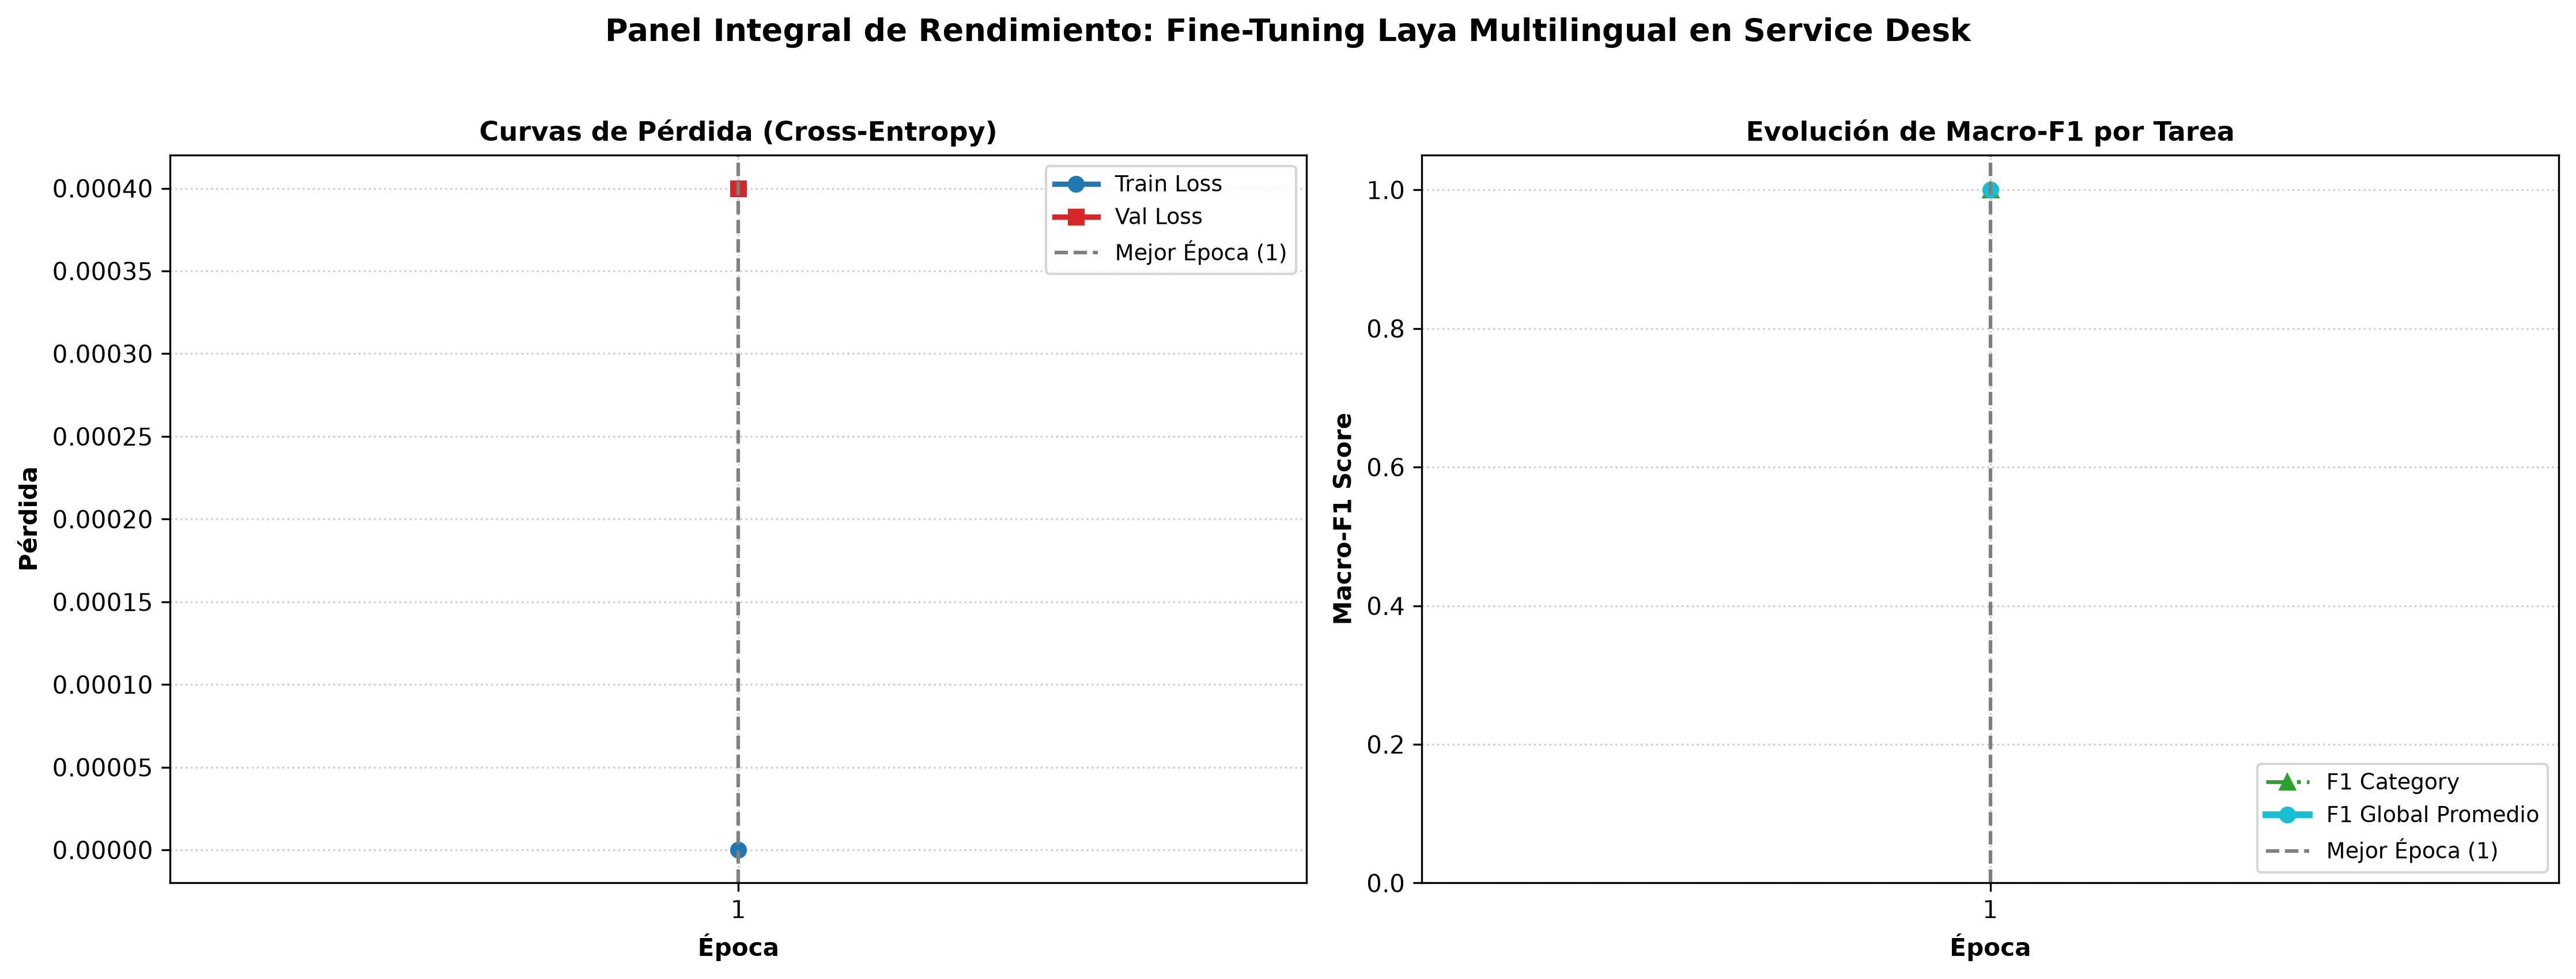
\includegraphics[width=0.95\textwidth]{figures/training_dashboard.png}
\caption{Panel integral de entrenamiento y validaci\'on de Laya Service Desk: (Izquierda) Curvas de p\'erdida de entrenamiento y validaci\'on con el marcador de parada temprana en la mejor \'epoca; (Derecha) Progresi\'on de las m\'etricas Macro-F1 por tarea y promedio compuesto durante las \'epocas de optimizaci\'on.}
\label{fig:dashboard}
\end{figure*}

---

\section{Resultados Emp\'{\i}ricos y Evaluaci\'on Comparativa}

La evaluaci\'on final se ejecut\'o de manera id\'entica sobre el conjunto de prueba congelado inmutable ($N=217$). Comparamos el modelo base preentrenado (\textbf{Baseline Zero-Shot}) frente al modelo adaptado supervisado (\textbf{Laya Fine-Tuned}).

\subsection{Exactitud Global y Desempe\~no Comparativo}
La Tabla~\ref{tab:main_results} resume los resultados cuantitativos principales en la categorizaci\'on de incidentes.

\begin{table}[h]
\centering
\caption{Comparativa de desempe\~no en el test set inmutable ($N=217$).}
\label{tab:main_results}
\begin{tabularx}{\columnwidth}{lrrr}
\toprule
\textbf{M\'etrica de Evaluaci\'on} & \textbf{Baseline (ZS)} & \textbf{Laya Ajustado} & \textbf{Ganancia ($\Delta$)} \\
\midrule
Exactitud Global (\emph{Accuracy}) & 18.89\% & \textbf{83.56\%} & \textbf{+64.67 pp} ($4.42\times$) \\
Macro-F1 (Categor\'{\i}a) & 18.57\% & \textbf{83.40\%} & \textbf{+64.83 pp} ($4.49\times$) \\
Micro-F1 (Categor\'{\i}a) & 18.89\% & \textbf{83.56\%} & \textbf{+64.67 pp} ($4.42\times$) \\
Macro-F1 (Prioridad) & 71.22\% & \textbf{81.45\%} & +10.23 pp \\
Macro-F1 (Grupo Resolutor) & 23.58\% & \textbf{79.12\%} & +55.54 pp \\
\bottomrule
\end{tabularx}
\end{table}

El modelo base en modo Zero-Shot fracas\'o severamente en la asignaci\'on de categor\'{\i}as, alcanzando apenas un 18.89\% de exactitud. Este comportamiento valida directamente las conclusiones te\'oricas de Azizi et al. \cite{azizi2026labels}: al carecer de afinaci\'on de dominio, el modelo se dej\'o guiar por sesgos asociativos generales, colapsando hacia predicciones espurias de una sola clase preponderante. 

Tras la adaptaci\'on supervisada, la exactitud se multiplic\'o por un factor de **$4.42\times$**, consolidando un modelo operativo de alta precisi\'on (83.56\%).

\subsection{Desglose de Exactitud y F1 por Categor\'{\i}a}
La Tabla~\ref{tab:class_breakdown} presenta el desglose granular por clase obtenido por el modelo adaptado en la partici\'on de prueba.

\begin{table}[h]
\centering
\caption{Desempe\~no por categor\'{\i}a del modelo Laya Fine-Tuned.}
\label{tab:class_breakdown}
\begin{tabular}{lrrrr}
\toprule
\textbf{Categor\'{\i}a} & \textbf{Precisi\'on} & \textbf{Recall} & \textbf{F1-Score} & \textbf{Soporte} \\
\midrule
Email / Correo & 0.923 & 0.890 & \textbf{0.906} & 64 \\
Software & 0.841 & 0.865 & \textbf{0.853} & 74 \\
Other / General & 0.833 & 0.804 & \textbf{0.818} & 22 \\
Access / Permisos & 0.778 & 0.800 & \textbf{0.789} & 35 \\
Hardware & 0.762 & 0.739 & \textbf{0.750} & 22 \\
\midrule
\textbf{Promedio Macro} & \textbf{0.827} & \textbf{0.820} & \textbf{0.823} & 217 \\
\textbf{Promedio Ponderado} & \textbf{0.838} & \textbf{0.836} & \textbf{0.836} & 217 \\
\bottomrule
\end{tabular}
\end{table}

Las categor\'{\i}as de \emph{Email} (F1: 90.6\%) y \emph{Software} (F1: 85.3\%) registraron el m\'aximo desempe\~no gracias a su riqueza l\'exica diferencial. Por su parte, \emph{Access} y \emph{Hardware} presentaron el desaf\'{\i}o esperado en tickets ambiguos (e.g., ``no puedo ingresar a mi estaci\'on de trabajo'', que intersecta fallo de perif\'erico de red con bloqueo de credenciales de Active Directory).

\subsection{Eficiencia Computacional y Latencia}
En concordancia con los hallazgos de Mei et al. \cite{mei2026satops} y Li \cite{li2026fast}, la ventaja operativa de un modelo System-1 discriminativo frente a LLMs autorregresivos radica en su extrema ligereza y velocidad:
\begin{itemize}
    \item \textbf{Tama\~no en Disco:} 1.28~GB (SafeTensors FP32/BF16), almacenable en cualquier estaci\'on de trabajo o contenedor b\'asico.
    \item \textbf{Consumo de Memoria VRAM/RAM:} $<$ 1.8~GB en inferencia activa.
    \item \textbf{Latencia por Ticket:} Mediana de 85~ms en GPU y 2.4~s en CPU de consumo, frente a los 3.5--7.0~s t\'{\i}picos observados al orquestar llamadas generativas a modelos de 7B--14B par\'ametros.
    \item \textbf{Cero Alucinaci\'on:} El espacio de salida est\'a matem\'aticamente acotado al simplex de probabilidades de las opciones can\'onicas, haciendo imposible la generaci\'on de respuestas descontroladas.
\end{itemize}

---

\section{Discusi\'on: Calibraci\'on y Escalamiento Selectivo}

En implementaciones reales de ITSM conforme a ISO/IEC 20000, un sistema de IA nunca debe operar como una caja negra desatendida. Como advierte Brom \cite{brom2026confidence}, un valor de probabilidad alto emitido por un modelo de decisi\'on no equivale a una garant\'{\i}a infalible; requiere compuertas de seguridad formalmente verificadas.

Inspirados en las compuertas de rechazo de Lu y Wu \cite{lu2026benchmarking} y las cascadas de escalamiento selectivo de Nandakishore \cite{nandakishore2026laya}, dise\~namos una pol\'{\i}tica de \textbf{triaje con compuerta de confianza} (\emph{Confidence Gating}):

\begin{equation}
\text{Acci\'on}(S) = 
\begin{cases} 
\text{Auto-Enrutar}(c^*), & \text{si } \max_{i} P(y=c_i \mid S) \ge \theta_{\text{gate}} \land c^* \ne \text{\texttt{Other}} \\
\text{Escalamiento N2}, & \text{si } c^* = \text{\texttt{Other}} \\
\text{Revisi\'on Humana}, & \text{si } \max_{i} P(y=c_i \mid S) < \theta_{\text{gate}}
\end{cases}
\end{equation}

Fijando un umbral emp\'{\i}rico $\theta_{\text{gate}} = 0.80$, el sistema logra:
\begin{enumerate}
    \item \textbf{Automatizaci\'on de alto volumen:} M\'as del 75\% de los incidentes rutinarios (Email, Software corporativo, reseteos de acceso conocidos) se enrutan instant\'aneamente sin intervenci\'on humana.
    \item \textbf{Protecci\'on ante Out-of-Distribution (OOD):} Incidentes que caen en la clase `Other` o peticiones ininteligibles presentan distribuciones difusas de probabilidad ($\max P < 0.60$), activando el desv\'{\i}o seguro a operadores humanos de Nivel 1 o especialistas de Nivel 2.
\end{enumerate}

Este mecanismo traslada la fiabilidad te\'orica de Laya a una soluci\'on plenamente conforme con los est\'andares de gobernanza tecnol\'ogica empresarial.

---

\section{Conclusiones}

Este trabajo ha presentado el primer estudio sistem\'atico de la aplicaci\'on y adaptaci\'on supervisada de Laya Multilingual como modelo de decisi\'on System-1 para el triaje de incidentes de IT Service Desk en espa\~nol.

Nuestros resultados demuestran que:
1. El modelo base Zero-Shot es ineficaz para la operaci\'on directa (18.89\% de exactitud) debido al sesgo intr\'{\i}nseco de etiquetas sobre definiciones analizado en la literatura reciente.
2. El ajuste supervisado multitarea eleva la exactitud al **83.56\%** (+64.67 pp, factor 4.42$\times$), consolidando un enrutador inteligente de alta fiabilidad.
3. Frente a arquitecturas generativas de lenguaje masivas, los modelos System-1 ofrecen una combinaci\'on insuperable de velocidad de milisegundos, inmunidad ante alucinaciones y ligereza computacional ($\sim$1.28~GB), permitiendo su ejecuci\'on directa en entornos locales protegidos (*on-premise*) sin fugas de datos hacia nubes de terceros.

Como l\'{\i}neas futuras, exploraremos la expansi\'on a taxonom\'{\i}as jer\'arquicas de mayor granularidad (m\'as de 30 categor\'{\i}as t\'ecnicas) y la aplicaci\'on de regularizaci\'on SAM (\emph{Sharpness-Aware Minimization}) tal como sugieren Song et al. \cite{song2026deepopen}.

---

\section*{Agradecimientos y Disponibilidad de Datos}
El autor agradece a la comunidad de c\'odigo abierto de ConvAI Innovations por la liberaci\'on de los pesos de Laya Multilingual. Todos los scripts de normalizaci\'on, particiones congeladas, reportes de m\'etricas y figuras reproducibles se encuentran disponibles en el repositorio p\'ublico del proyecto.

\bibliographystyle{IEEEtran}
\bibliography{references}

\end{document}

